\documentclass[border=8pt]{standalone}
\usepackage{tikz}
\usetikzlibrary{arrows.meta, positioning, calc}

% Persona accent colours (Okabe-Ito, colourblind-safe)
\definecolor{maximiser}{HTML}{0072B2}     % blue
\definecolor{differentiator}{HTML}{009E73} % teal
\definecolor{newcoder}{HTML}{D55E00}       % vermillion
\definecolor{sceptic}{HTML}{CC79A7}        % rose
\definecolor{juggler}{HTML}{E69F00}        % orange
\definecolor{weekblue}{HTML}{56B4E9}       % sky

% Colours matched to the light site palette (Catppuccin Latte)
\colorlet{txtmain}{black}
\colorlet{txtmuted}{black!55}
\colorlet{cardfill}{white}
\definecolor{cardborder}{HTML}{CCCCCC}
\colorlet{cardtext}{black!75}
\colorlet{flowfill}{weekblue!8}
\colorlet{flowtext}{black}

\begin{document}
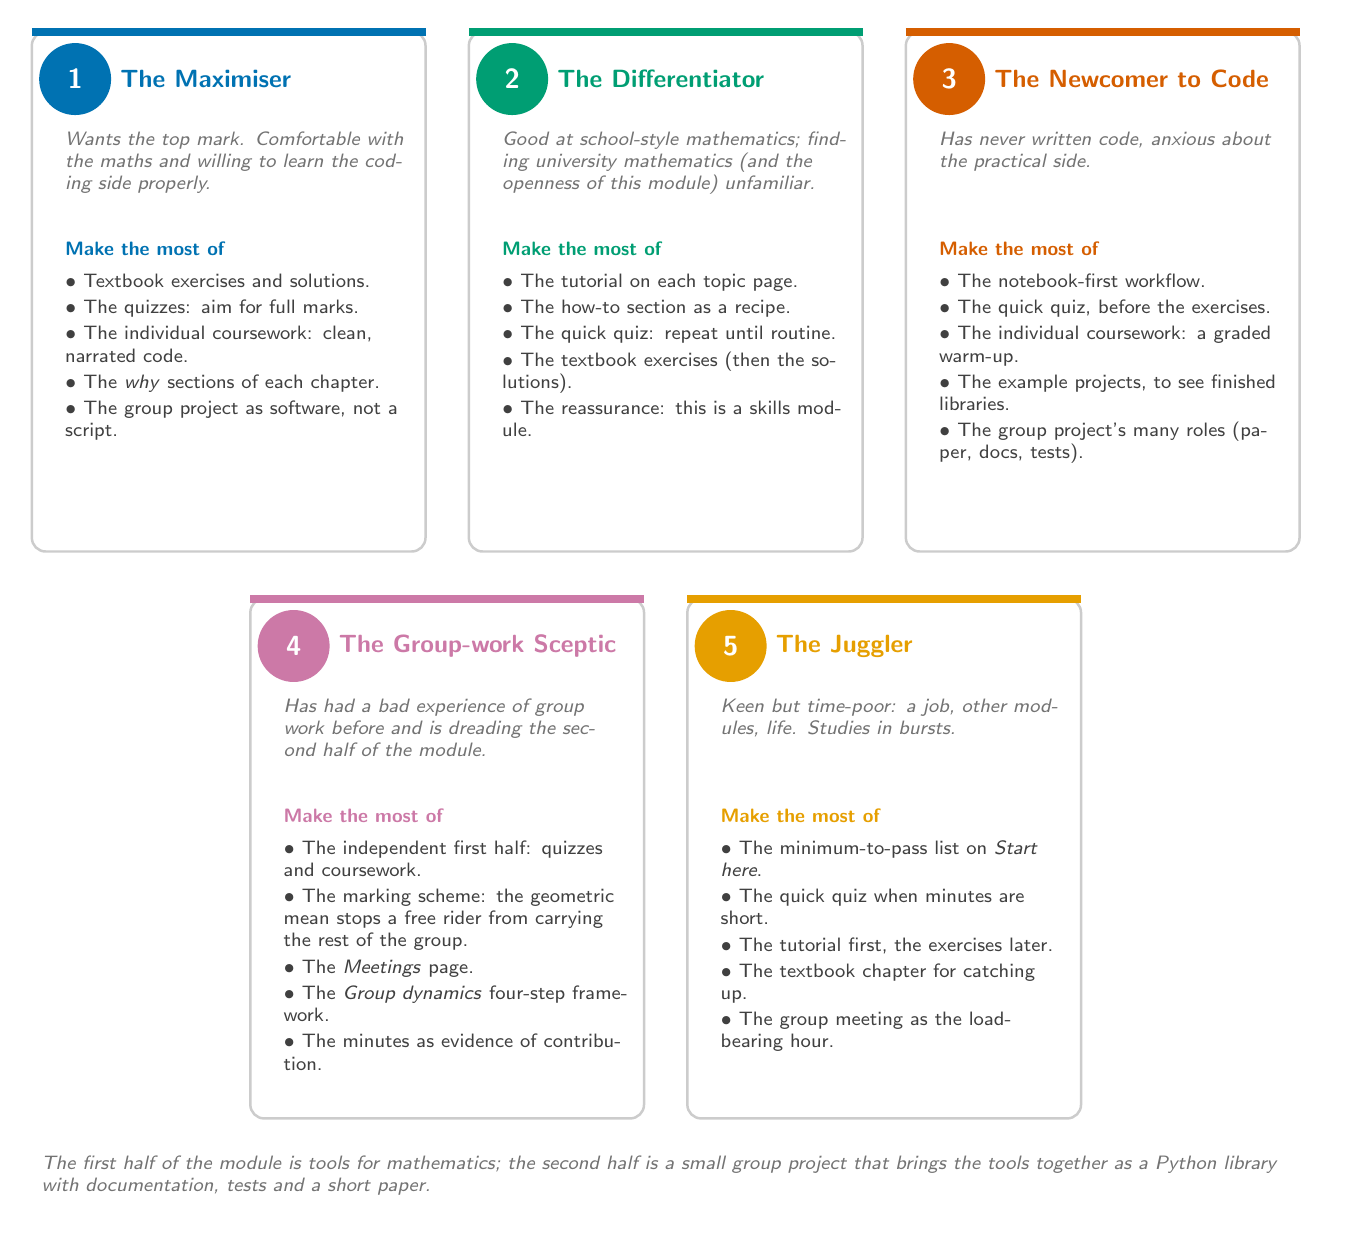
\begin{tikzpicture}[
    font=\sffamily,
    >=Stealth,
    icon/.style={circle, minimum size=26pt, inner sep=0pt, text=white,
                 font=\sffamily\normalsize\bfseries},
    ptitle/.style={font=\sffamily\small\bfseries, anchor=west},
    pdesc/.style={font=\sffamily\scriptsize\itshape, text=txtmuted,
                  align=left, text width=4.4cm, anchor=north west},
    head/.style={font=\sffamily\scriptsize\bfseries, anchor=north west},
    item/.style={font=\sffamily\scriptsize, text=cardtext,
                 align=left, text width=4.4cm, anchor=north west},
]

\def\pw{5.0}
\def\ph{6.6}
\def\gap{0.55}
\def\rowtwo{0}
\def\rowone{7.2}

% Persona card macro: #1 x, #2 y, #3 colour, #4 num, #5 title,
%                    #6 descriptor, #7 heading, #8 items
\newcommand{\personacard}[8]{
    \begin{scope}[shift={(#1, #2)}]
        \draw[rounded corners=5pt, draw=cardborder, line width=0.9pt, fill=cardfill]
            (0, 0) rectangle (\pw, \ph);
        \draw[#3, line width=3pt, rounded corners=5pt]
            (0.0, \ph) -- (\pw, \ph);
        \node[icon, fill=#3] at (0.55, \ph-0.6) {#4};
        \node[ptitle, text=#3] at (1.0, \ph-0.6) {#5};
        \node[pdesc] at (0.3, \ph-1.15) {#6};
        \node[head, text=#3] at (0.3, \ph-2.55) {#7};
        \node[item] at (0.3, \ph-2.95) {#8};
    \end{scope}
}

% TOP ROW of personas
\personacard{0}{\rowone}{maximiser}{1}{The Maximiser}
    {Wants the top mark. Comfortable with the maths and willing to learn the
    coding side properly.}
    {Make the most of}
    {%
        $\bullet$ Textbook exercises and solutions.\\[1.5pt]
        $\bullet$ The quizzes: aim for full marks.\\[1.5pt]
        $\bullet$ The individual coursework: clean, narrated code.\\[1.5pt]
        $\bullet$ The \emph{why} sections of each chapter.\\[1.5pt]
        $\bullet$ The group project as software, not a script.%
    }

\personacard{\pw+\gap}{\rowone}{differentiator}{2}{The Differentiator}
    {Good at school-style mathematics; finding university mathematics (and
    the openness of this module) unfamiliar.}
    {Make the most of}
    {%
        $\bullet$ The tutorial on each topic page.\\[1.5pt]
        $\bullet$ The how-to section as a recipe.\\[1.5pt]
        $\bullet$ The quick quiz: repeat until routine.\\[1.5pt]
        $\bullet$ The textbook exercises (then the solutions).\\[1.5pt]
        $\bullet$ The reassurance: this is a skills module.%
    }

\personacard{2*\pw+2*\gap}{\rowone}{newcoder}{3}{The Newcomer to Code}
    {Has never written code, anxious about the practical side.}
    {Make the most of}
    {%
        $\bullet$ The notebook-first workflow.\\[1.5pt]
        $\bullet$ The quick quiz, before the exercises.\\[1.5pt]
        $\bullet$ The individual coursework: a graded warm-up.\\[1.5pt]
        $\bullet$ The example projects, to see finished libraries.\\[1.5pt]
        $\bullet$ The group project's many roles (paper, docs, tests).%
    }

% BOTTOM ROW of personas (two cards, centred)
\personacard{2.775}{\rowtwo}{sceptic}{4}{The Group-work Sceptic}
    {Has had a bad experience of group work before and is dreading the second
    half of the module.}
    {Make the most of}
    {%
        $\bullet$ The independent first half: quizzes and coursework.\\[1.5pt]
        $\bullet$ The marking scheme: the geometric mean stops a free rider
        from carrying the rest of the group.\\[1.5pt]
        $\bullet$ The \emph{Meetings} page.\\[1.5pt]
        $\bullet$ The \emph{Group dynamics} four-step framework.\\[1.5pt]
        $\bullet$ The minutes as evidence of contribution.%
    }

\personacard{8.325}{\rowtwo}{juggler}{5}{The Juggler}
    {Keen but time-poor: a job, other modules, life. Studies in bursts.}
    {Make the most of}
    {%
        $\bullet$ The minimum-to-pass list on \emph{Start here}.\\[1.5pt]
        $\bullet$ The quick quiz when minutes are short.\\[1.5pt]
        $\bullet$ The tutorial first, the exercises later.\\[1.5pt]
        $\bullet$ The textbook chapter for catching up.\\[1.5pt]
        $\bullet$ The group meeting as the load-bearing hour.%
    }

% Footer note
\node[font=\sffamily\scriptsize\itshape, text=txtmuted, anchor=north west,
      text width=16.1cm]
    at (0, -0.35)
    {The first half of the module is tools for mathematics; the second half
     is a small group project that brings the tools together as a Python
     library with documentation, tests and a short paper.};

\end{tikzpicture}
\end{document}
